\documentclass[border=12pt]{standalone}
\def\pgfsysdriver{pgfsys-dvisvgm.def}
\usepackage[dvisvgm]{xcolor}
\usepackage{xeCJK}
\setCJKmainfont{HaranoAjiGothic-Regular.otf}[BoldFont=HaranoAjiGothic-Bold.otf]
\setCJKsansfont{HaranoAjiGothic-Regular.otf}[BoldFont=HaranoAjiGothic-Bold.otf]
\usepackage{amsmath,amssymb,tikz,lmodern}
\usetikzlibrary{arrows.meta,positioning,calc,fit,backgrounds}
\renewcommand{\familydefault}{\sfdefault}
\definecolor{ink}{HTML}{25322F}
\definecolor{green}{HTML}{246657}
\definecolor{tint}{HTML}{EEF4F0}
\definecolor{soft}{HTML}{C6D2CC}
\definecolor{muted}{HTML}{52615B}
\newif\ifJapanese
\newcommand{\Tx}[2]{\ifJapanese #1\else #2\fi}
\newcommand{\Eff}{\overline{\operatorname{Eff}}}
\newcommand{\heading}[3]{{\color{green}\bfseries #1\quad\Tx{#2}{#3}}\\[5pt]}
% A white rectangle makes the complete citation label clickable, including spaces.
\newcommand{\refurl}[2]{\special{dvisvgm:raw <a xlink:href="#1" target="_blank" rel="noopener noreferrer">}{\setlength{\fboxsep}{0pt}\colorbox{white}{\color{green}\underline{\strut #2}}}\special{dvisvgm:raw </a>}}
\tikzset{
 card/.style={draw=soft,fill=white,rounded corners=2pt,align=left,text=ink,font=\fontsize{10.5}{14}\selectfont,inner xsep=12pt,inner ysep=10pt,text width=14.4cm},
 half/.style={card,text width=6.45cm,minimum height=2.05cm},
 result/.style={card,draw=green,fill=tint,line width=.9pt},
 reason/.style={align=left,text=muted,font=\fontsize{9}{12}\selectfont,inner sep=0pt,text width=12.7cm},
 branchreason/.style={reason,text width=5.95cm},
 edge/.style={-{Stealth[length=2.4mm]},draw=green,line width=1pt},
 wire/.style={draw=green,line width=1pt},
}
% Keep the arrow in a dedicated left gutter; explanations never cover it.
\newcommand{\flow}[3]{
 \coordinate (#2-from) at ($(#1.south)+(-6.9,0)$);
 \coordinate (#2-to) at ($(#2.north)+(-6.9,0)$);
 \draw[edge] (#2-from)--(#2-to);
 \node[reason,anchor=west] (#2-reason) at ($(#2-from)!.5!(#2-to)+(.55,0)$) {#3};
}

\newcommand{\Cite}[2]{\refurl{#1}{#2}}

\Japanesetrue
\begin{document}
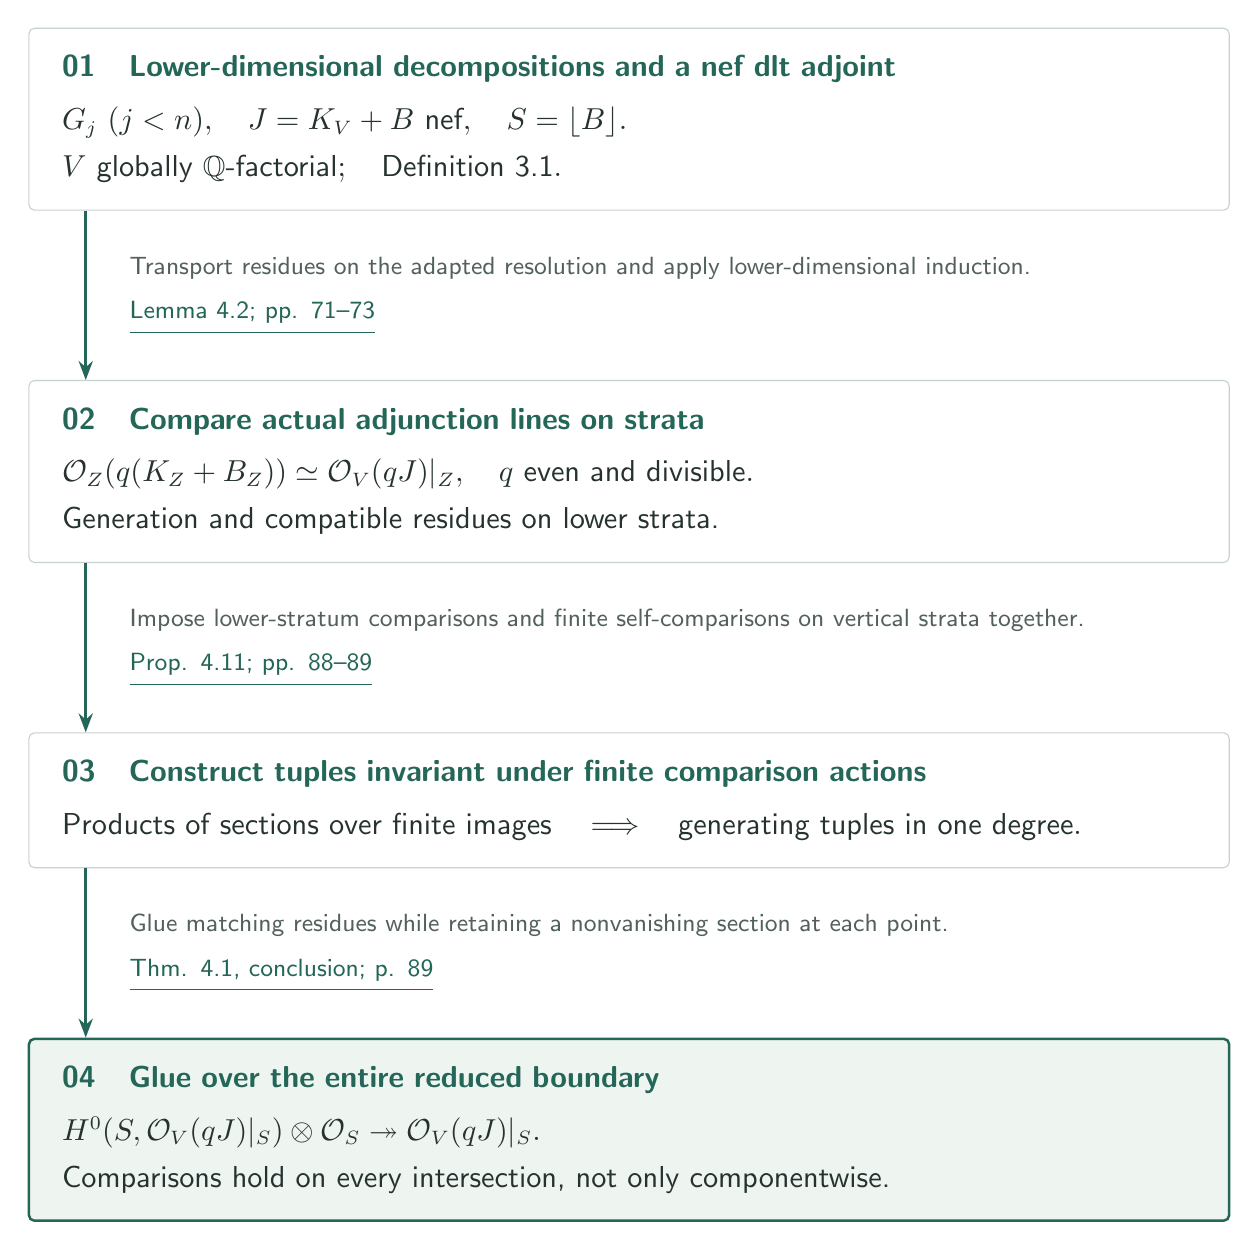
\begin{tikzpicture}
\node[card] (n0) {\heading{01}{下の次元の分解とnefなdlt随伴因子}{Lower-dimensional decompositions and a nef dlt adjoint}$G_j\ (j<n),\quad J=K_V+B\text{ nef},\quad S=\lfloor B\rfloor.$\\[3pt] $V\text{ globally }\mathbb Q\text{-factorial};\quad\text{Definition 3.1}.$};
\node[card,below=2.15cm of n0] (n1) {\heading{02}{stratum上の実際の随伴直線束を比較する}{Compare actual adjunction lines on strata}$\mathcal O_Z(q(K_Z+B_Z))\simeq\mathcal O_V(qJ)|_Z,\quad q\text{ even and divisible}.$\\[3pt] $\Tx{\text{下位stratumでの生成と留数の整合性。}}{\text{Generation and compatible residues on lower strata.}}$};
\flow{n0}{n1}{\Tx{lc strataに適合した解消で留数を運び、低次元の帰納を適用。}{Transport residues on the adapted resolution and apply lower-dimensional induction.}\\[4pt]\Cite{https://github.com/openai/math/blob/adc7f1241b42e322a6451854ab7e4b4c146bf78a/preprints/Log-abundance-for-compact-Kahler-spaces-under-logarithmic-Iitaka-subadditivity-October-4-2026/main.pdf}{Lemma 4.2; pp. 71--73}}
\node[card,below=2.15cm of n1] (n2) {\heading{03}{有限な比較作用に対して不変tupleを作る}{Construct tuples invariant under finite comparison actions}$\Tx{\text{有限像に沿う切断の積}}{\text{Products of sections over finite images}}\quad\Longrightarrow\quad\Tx{\text{共通次数の生成tuple}}{\text{generating tuples in one degree}}.$};
\flow{n1}{n2}{\Tx{下位strataの比較と、垂直strataの自己比較の有限像を同時に処理。}{Impose lower-stratum comparisons and finite self-comparisons on vertical strata together.}\\[4pt]\Cite{https://github.com/openai/math/blob/adc7f1241b42e322a6451854ab7e4b4c146bf78a/preprints/Log-abundance-for-compact-Kahler-spaces-under-logarithmic-Iitaka-subadditivity-October-4-2026/main.pdf}{Prop. 4.11; pp. 88--89}}
\node[result,below=2.15cm of n2] (n3) {\heading{04}{被約境界全体へ貼り合わせる}{Glue over the entire reduced boundary}$H^0(S,\mathcal O_V(qJ)|_S)\otimes\mathcal O_S\twoheadrightarrow\mathcal O_V(qJ)|_S.$\\[3pt] $\Tx{\text{各成分だけでなく、全ての交差上の比較も満たす。}}{\text{Comparisons hold on every intersection, not only componentwise.}}$};
\flow{n2}{n3}{\Tx{整合する留数を貼り合わせ、各点で非消滅な切断を残す。}{Glue matching residues while retaining a nonvanishing section at each point.}\\[4pt]\Cite{https://github.com/openai/math/blob/adc7f1241b42e322a6451854ab7e4b4c146bf78a/preprints/Log-abundance-for-compact-Kahler-spaces-under-logarithmic-Iitaka-subadditivity-October-4-2026/main.pdf}{Thm. 4.1, conclusion; p. 89}}
\end{tikzpicture}

\end{document}
